%! TEX root = **/000-main.tex
% vim: spell spelllang=en:

\section{Introdução}%
\label{sec:introduction}
Na área da computação um benchmark refere-se a execução de um programa ou conjunto de programas com o intuito de avaliar o desempenho relativo de algo, ou também pode ser sinônimo do programa ou conjunto de programas usados para tal.


O propósito de um benchmark é permitir a comparação das perfomances relativas de diferentes sistemas sem depender exclusivamente das especificações do mesmo, que podem ser difíceis de comparar e, por conseguinte levar a conclusões errôneas.

Ao falar especificamente de benchmarks de processadores diversas metricas surgiram através do tempo, como MIPS (Mega Instructions Per Second), MOPS (Mega Operations Per Second), MFLOPS (Mega FLoating point Opetarions Per Second), MHz (Mega Hertz), tendo cada uma dessas metricas sua importância histórica e periodo de uso. Entretanto das metricas apresentadas as que serão discutidas e comparadas nas sessões seguintes serão MIPS e MFLOPS.

\begin{figure}[H]
    \centering
    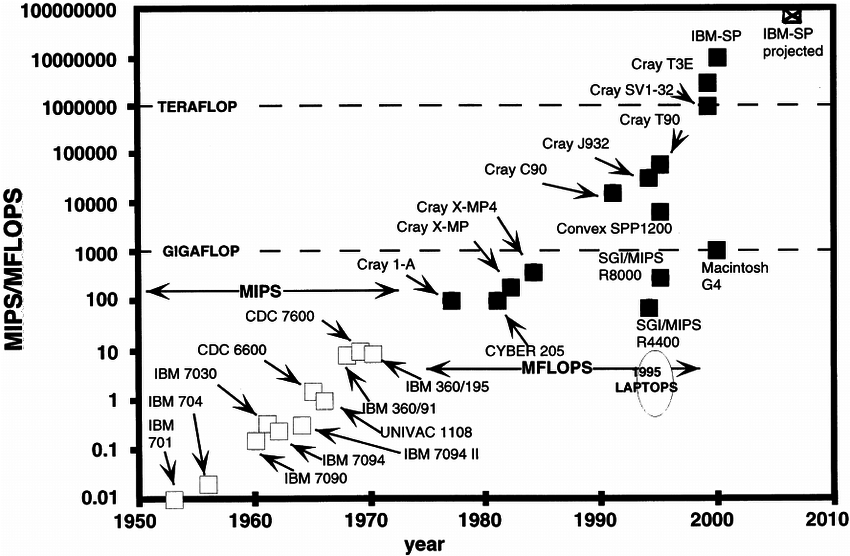
\includegraphics[height=6cm]{performanceOvertimeChart}
    \caption{
        Development of computer power since 1950. Speeds are shown in millions of instructions per second (MIPS) up to 1974 and in millions of floating point operations per second (MFLOPS) from 1975 onwards. The rate of increase is exponential and shows no signs of tailing off, from \cite{mcguffie_henderson-sellers}.
    }
\end{figure}
 
